
Töö planeerimisel ei olnud esialgu selge, kuidas täpselt töö valmima peaks. Autoril puudus nii otsene kui kaudne kokkupuude suurte andmebaaside loomise ja haldamisega. Seetõttu kaasnes tööga palju katseid ja ka läbikukkumisi. Siin peatükkis on kirjeldatud, kuidas jõuti lõpptulemuseni.

\section{Lahenduse arhitektuur} %This creates a new subsection titled 
\begin{figure}[h!]
    \centering
    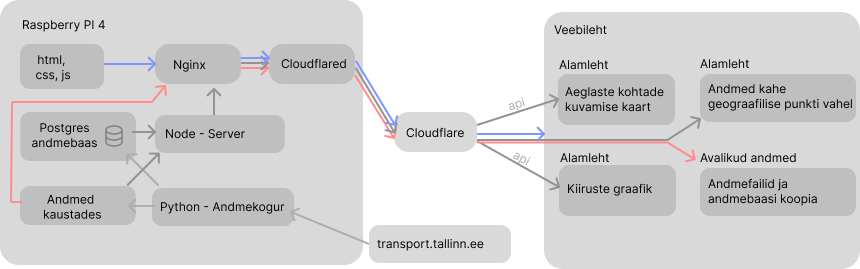
\includegraphics[width=0.95\textwidth]{figures/struktuur.png}
    \caption{Arhitektuuriline lahendus.}
    \label{fig:Struktuur}
\end{figure}

Joonisel \ref{fig:Struktuur} on näha, kuidas andmed kogutakse \url{transport.tallinn.ee} kaudu. Andmete kogumiseks on kirjutatud Pythoni skript. Geograafilised asukohad salvestatakse andmebaasi, muud andmed salvestatakse kaustadesse. Kui kasutaja avab veebilehe, siis turvalisuse tagamiseks on kasutusel Cloudflare nimeline teenus. Kogu suhtlus käib läbi Cloudflare serveri, see tähendab, et Raspberry Pi  IP-aadress ei ole avalik. Lokaalselt on kasutusel Node server, mis teeb päringuid PostgreSQL andmebaasi pihta.

\section{Andmete päritolu}


Enne andmete kogumist tuli kaardistada kohad, kust andmeid on võimalik koguda. Selleks uuriti, kust saab andmed Tallinna ühistranspordi leht \footnote{\url{https://transport.tallinn.ee/}} ja vaadati üldiselt internetis ringi, et kas leidub veel kohti.
Tõenäoliselt ei ole Tabel \ref{tab:andmeteAsukohad} tulem täielik.

\begin{longtable}[hp]{|p{5cm}|p{4cm}|p{2cm}|p{2cm}|} % Begins a longtable with three columns, defining specific widths for each column
	\caption{Kohad kust andmeid koguda.} % Provides a caption for the table, italicizing the text
	\label{tab:andmeteAsukohad}\\ \hline % Sets a label for the table and starts the table with a horizontal line
	\textbf{URL} &  \textbf{Andmeliik} & \textbf{Andmetüüp} & \textbf{Töös kogutud}  \\ % Table header with bold text
	\hline % Adds a horizontal line after the header
	\endfirsthead % Marks the end of the header for the first page of the table
	\multicolumn{3}{l} % Merges three columns for the continuation note
	{\tablename\ \thetable\ -- \textit{Jätkub...}} \\ % Creates a continuation note with italicized text
	\hline
	\textbf{URL} &  \textbf{Andmeliik} & \textbf{Andmetüüp} & \textbf{Töös kogutud}   \\  % Table header for continued pages, with bold text
	\hline
	\endhead % Marks the end of the header for all pages after the first
	\hline \multicolumn{3}{l}{\textit{Jätkub...}} \\ % Adds a note at the end of the table for continued pages
	\endfoot % Marks the end of the table body
	\hline
	\endlastfoot % Marks the end of the table for the last page
 \url{https://transport.tallinn.ee/gps.txt} & Reaalajas asukohad & CSV & Ei\\ \hline 
\url{https://transport.tallinn.ee/ readfile.php?name=gps.txt} & Reaalajas asukohad & CSV & Jah, iga 30s tagant\\ \hline
\url{https://gis.ee/tallinn/gps.php} & Reaalajas asukohad & JSON & Ei\\ \hline

 \url{https://transport.tallinn.ee/data/tallinna-linn\_bus\_18.txt} & Ühissõidukite marsruudid (iga marsruut eraldi) & TXT & Jah, kord päevas kell 04:00\\
\hline 
\url{https://transport.tallinn.ee/data/routes.txt} & Ühissõidukite sõiduplaanid & TXT &Jah, kord päevas kell 04:00\\
\hline 
\url{https://transport.tallinn.ee/data/stops.xml} & Peatuste asukohad & XML & Jah, kord päevas kell 04:00\\
\hline 
\url{https://transport.tallinn.ee/tabloconfig2021.php} & Ebaselge, kuid paistab kuvavat infot juhul kui väljumist ei toimu, kuid mitte alati & JSON & Ei\\
\hline
\url{https://transport.tallinn.ee/interruptions.json} & Ootamatud tõrked & JSON & Jah, iga 5 minuti tagant\\
\hline 
\url{https://transport.tallinn.ee/announcements.json} & Teadaanded & JSON & Jah, kord päevas kell 04:00\\
\hline
\url{https://transport.tallinn.ee/data/gtfs.zip} & Tallinna GTFS formaadis andmed  & ZIP & Jah, kord päevas alates aprill 2025\\
\hline
\url{https://www.peatus.ee/gtfs/gtfs.zip} & Eesti GTFS formaadis andmed  & ZIP & Ei\\
\hline
\end{longtable}
\newpage
Antud tabeli puhul on oluline märkida, et kohad, kust andmeid koguti, muutusid ajas. Seda seetõttu, kuna töö käigus avastati uusi kohti. Näiteks 2025 kevadel leiti koht, kust laadida Tallinnat puudutav info ühest kohast ühe failina \footnote{\url{https://transport.tallinn.ee/data/gfts.zip}}. Kogu Eesti andmeid ei kogutud, kuna see polnud töö eesmärk. Reaalaajandmete puhul oli valikus mitu kohta, kust andmeid saada, kuid lõpuks jäädi praeguse lahenduse juurde, kuna sealt saadavatel andmetel oli lisatulp sihtkoha infoga.

Kuigi väiksed muudatused toimusid, siis lõplikult kogutakse järgmist infot:
\begin{enumerate}
    \item Reaalaajaandmed: aeg, liin, sõidukitüüp, asukoht, sihtpunkt, sõiduki identifikaator, suund.
    \item Teadaanded: liinide ja sõidugraafikute muudatused.
    \item Ootamatud tõrked: info tõrgete kohta.
    \item GTFS: peatuste asukohad, marsruudid, ajagraafikud jne.
    
\end{enumerate}



\section{Raspberry Pi serverina} % This creates a new section with the title "First Section of the First Chapter."
Raspberry Pi 4 on ühendatud 1-terabaidise kõvakettaga, mõlemat on näha Joonisel \ref{fig:RaspberryPi}. Seadistamiseks on kasutatud 64 GB mälukaarti, millele paigaldati \textit{Raspberry Pi OS Lite (64-bit)} operatsioonisüsteem.
Serveri töökindluse tagamiseks on seadistatud valvetimer (\textit{watchdog timer}), mis taaskäivitab süsteemi, kui see peaks kokku jooksma. Käivituse järel toimub automaatselt kõvakettaga ühendamine ja andmekogumise protsessi käivitamine.

\begin{figure}[h!]
    \centering
    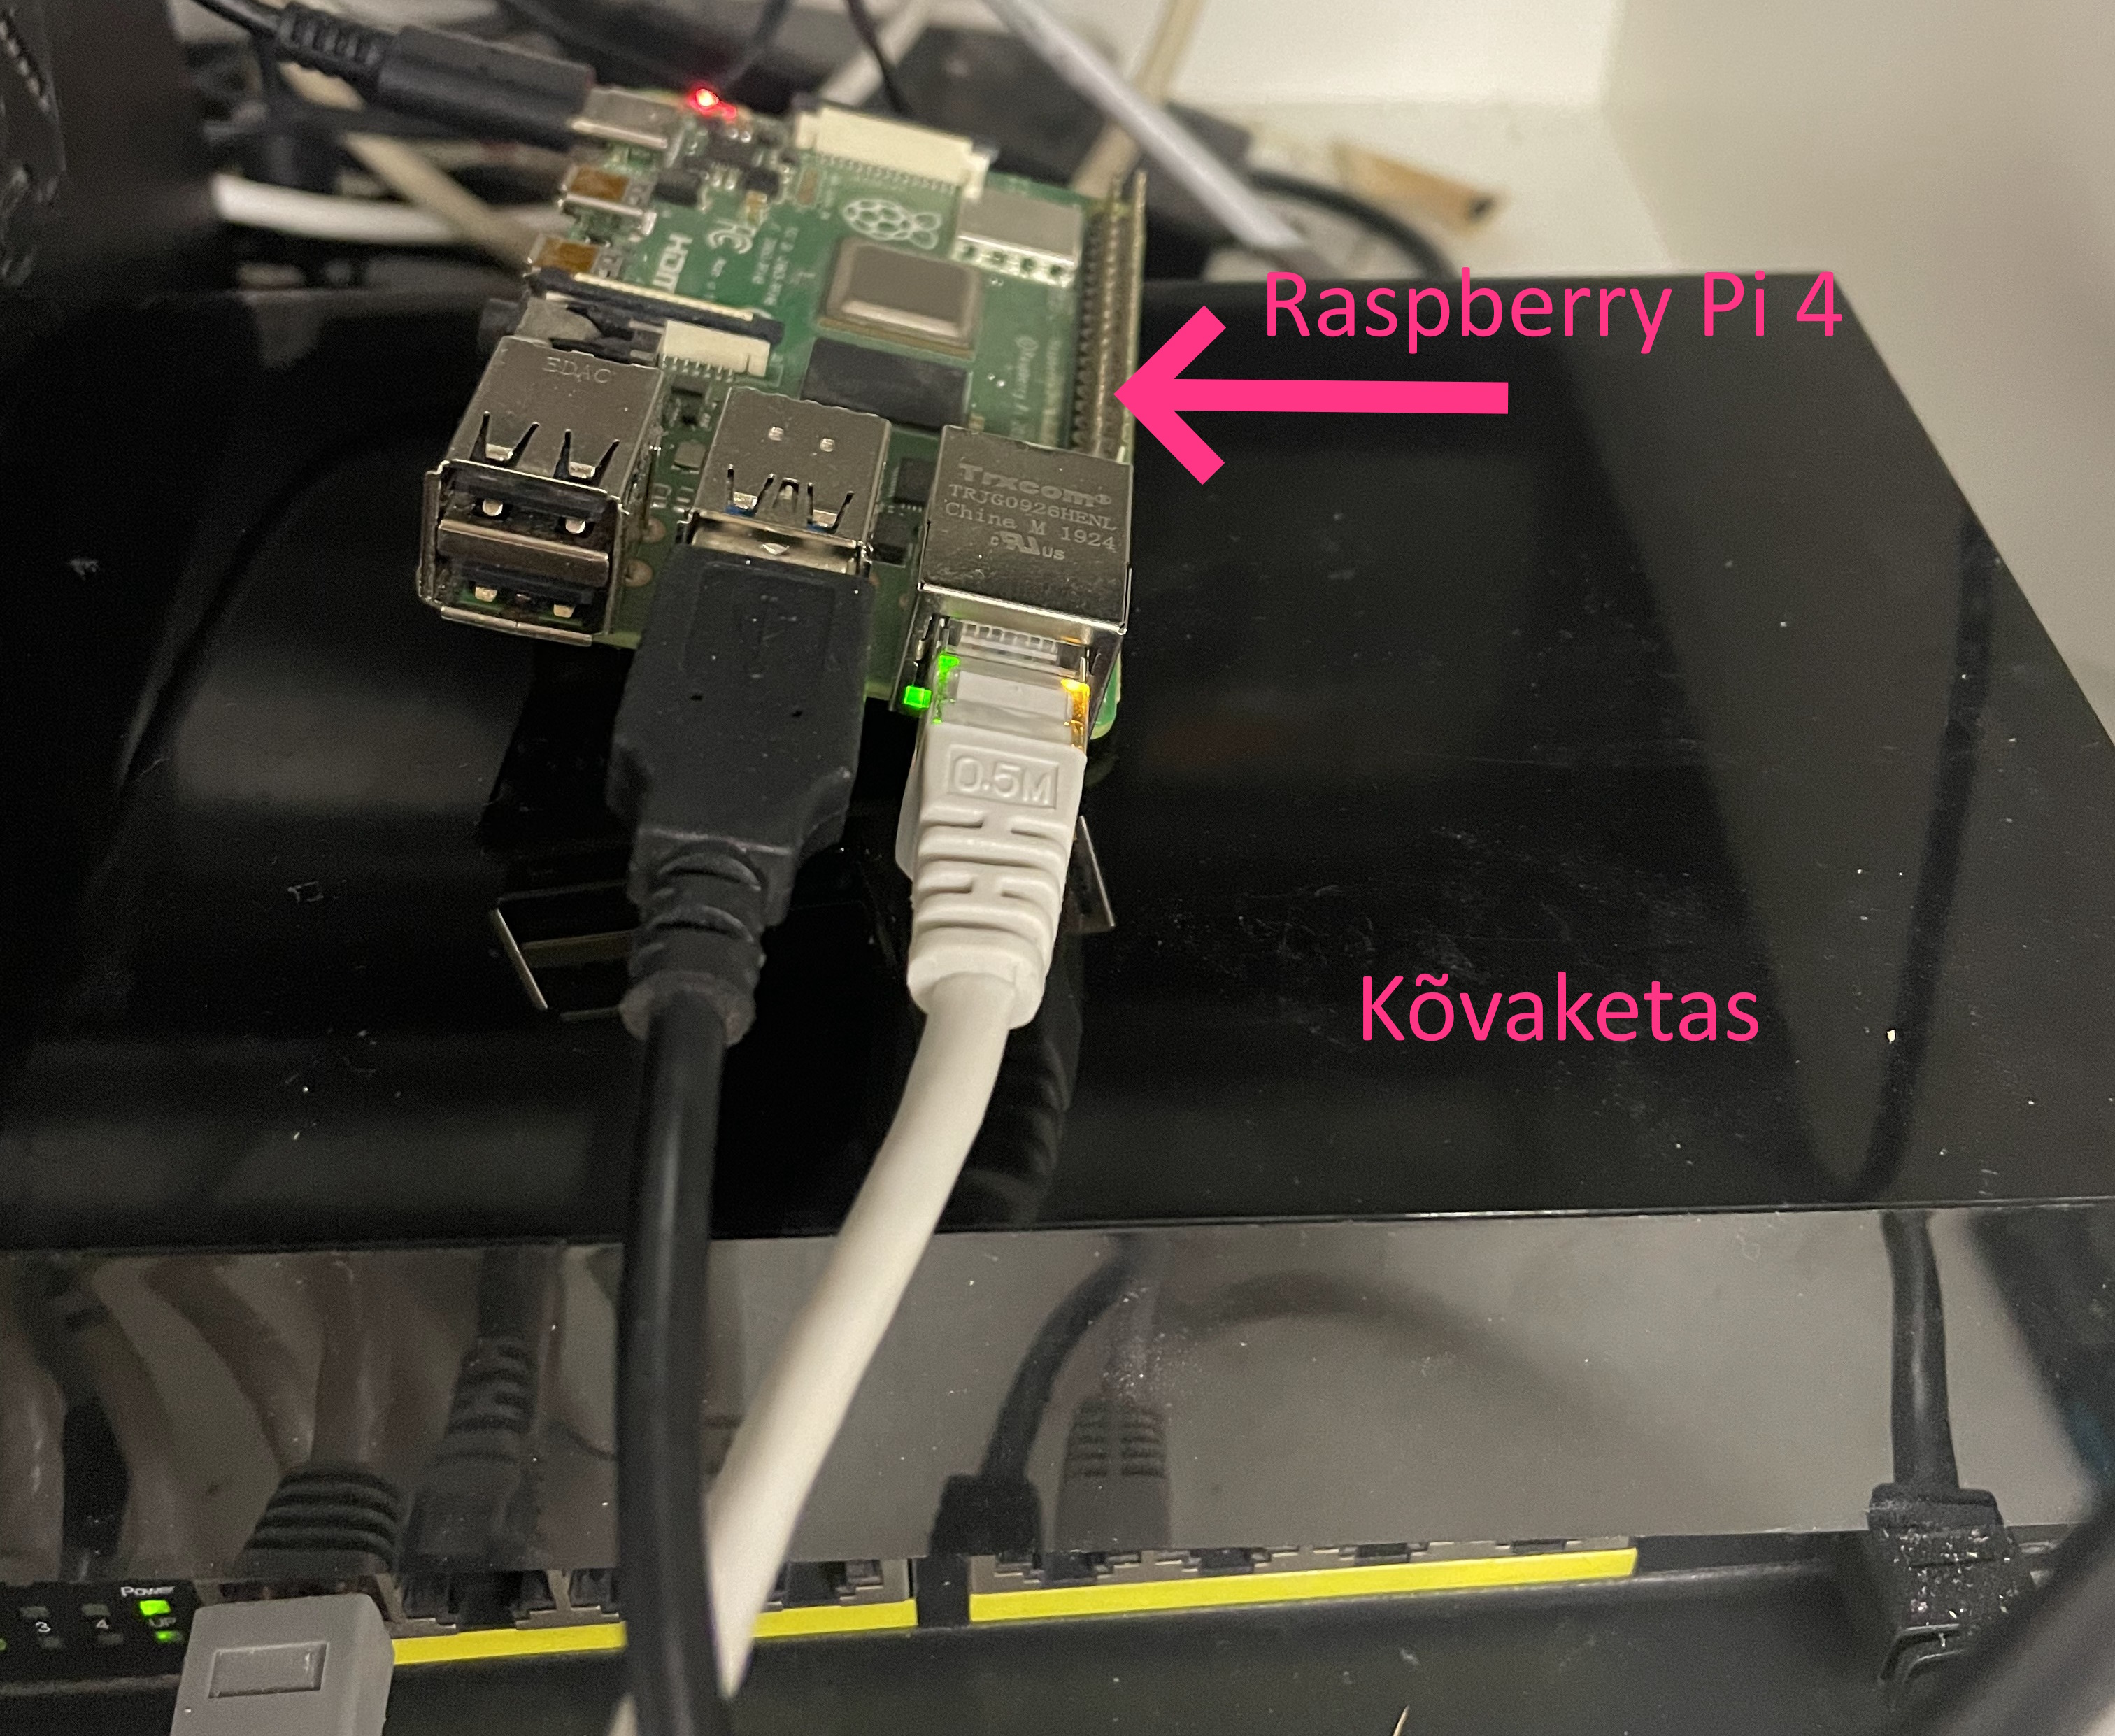
\includegraphics[width=0.45\textwidth]{figures/RaspberryPi.jpg}
    \caption{Rasberry Pi 4 ja kõvaketas autori kodus.}
    \label{fig:RaspberryPi}
\end{figure}

Raspberry Pi 4 ja kõvaketas valiti töö jaoks, kuna mõlemad olid autoril enne tööga alustamist juba olemas ja rahaliste väljaminekute vältimiseks otsustati neid ka kasutada. Teiste variantidena kaaluti lauaarvuti kasutamist, kuid oma suure suuruse ja müra tõttu tundus see ebapraktiline. Raspberry Pi oli ilma mürata ning selle sai paigutada kitsasse kappi. Kolmanda variandina kaaluti virtuaalse privaatse serveri kasutamist. Kuid nende puhul on üldjuhul tegu tasuliste teenustega \cite{Hetzner2025}, millel on rangemad piirangud kui enda hallataval serveril. Soov omada täielikku kontrolli serveri üle, hind ja eksperimenteerimise lihtsustamine jätsid pilvepõhise serveri valikust välja.



\section{Andmete kogumise skript} % This creates a new section with the title "First Section of the First Chapter."
Reaalaajaandmete kogumiseks on kirjutatud Pythonis skript, mida haldab \textit{systemd} ja mis käivitatakse \textit{systemctl} käsureatööriista abil teenusena. See võimaldab skripti automaatset käivitamist, tõrgete korral taaskäivitamist ning logide jälgimist.

Staatilisi andmeid kogutakse iga päev kell 04:00. Esialgu koguti andmeid selliselt nagu \url{transport.tallinn.ee} oma enda veebilehe siseseid päringuid tegi, mis tähendas, et osad andmed olid ebastandartsel kujul ja inimesele raskesti arusaadavad. Kõige suuremaid raskusi põhjustas autorile ajagraafiku failist \footnote{\url{https://tallinn.simplytobo.eu/transport_data/transport_data/bus_times_data/2025-06-04/routes.txt}} arusaamine, ning autor ei suutnudki seda lõpikult teha. See muutis teisele uurimusküsimusele ("Kui suured on liinil sõitvate sõidukite hilinemised?") vastuse leidmise väga ajanõudvaks. Alles töö lõpus leiti, et samal leheküljel eksisteeris ka paremini arusaadav fail.
 
Töö lõpus leiti, et \url{transport.tallinn.ee} lehel on olemas GTFS formaadis koht, kust saab heal kujul andmeid, sealhulgas ajagraafikuid. Autor lisas GTFS andmete kogumise loogika.  Selleks tehakse igal hommikul päring päise (\textit{header}) küsimiseks. Kui päises on rida (\textit{Last-Modified}), mis kirjeldab millal viimati andmeid muudetud, on vahepeal uuenenud, siis tehakse uus päring ja laetakse andmed päriselt alla. GTFS fail on  pigem väike (alla 10 MB), kuid hea tava on ikkagi laadida ainult siis, kui vajadus.

Iga päev saadab skript välja teate autorile sotsiaalmeedia platvormile Discord. Sõnum sisaldab infot selle kohta, kas andmete kogumine endiselt töötab ja kui palju andmeid eelmine päev salvestati. Juhul kui andmete salvestamine mingil põhjusel ebaõnnestub, siis selle kohta saadetakse koheselt veateade. See võimaldas autoril jälgida toimuvat telefonist ja mitmed vead avastati just nii.
 
\section{Andmete hoiustamine}

Andmete hoiustamiseks katsetati mitut viisi. Esialgu koguti kõiki andmeid kaustadesse. Andmed jaotati esialgu nende tüübi (6 kausta), siis kuupäeva (365 kausta aastas) ja siis salvestati fail selliselt, et kellaaeg oli nimeks. Antud viis töötas hästi, kui andmeid oli vähe. 

Reaalajaandmeid hakkas aja jooksul kogunema nii palju, et mitme päeva analüüsimine muutus väga aeglaseks. Samuti tuli kõik andmetega ümberkäivad funktsioonid nullist kirjutada. Pythoniga muutus see kiirelt liiga aeglaseks ja raskesti hallatavaks. Autor proovis kasutada komplileeritud keelt nagu Go ja kuigi seal oli andmetega ümberkäimine kordades kiirem, oli see endiselt raskesti hallatav. 

Juba 2024. sügisel valiti proovimiseks SQLite andmebaas. Seda seetõttu, kuna tol hetkel usuti, et selle jõudlusest piisab. Katsetuste käigus selgus, et andmete andmebaasi saamine on väga ajakulukas ning päringute tegemine on kohati aeglasem kui otse kaustast võtmine. Prooviti mitmeid optimeerimise viise. Näiteks andmebaasi kuu suurusteks tükkideks jagamist, ajatulba indekseerimist, andmebaasi tõstmist võimsama arvuti peale, kuid lõpuks muutus andmebaasiga ümberkäimine liialt ajakulukaks. Autor otsis seejärel uut viisi andmete hoiustamiseks.

Juhendaja soovitusel uuriti täpsemalt aegrea andmebaaside võimalusi. Valikuvariantide all olid InfluxDB, Prometheus, Graphite ja TimescaleDB. Valiku tegemine oli raske, kuid lõpuks otsustati TimescaleDB kasuks. Seda nimelt seetõttu, et tegu on PostgreSQL andmebaasi lisaga. PostgreSQL on aga üks kõige populaarsemaid andmebaasihaldussüsteeme \cite{dbengines_ranking}. See tähendab head dokumentatsiooni, kuidas asju teha. Täpsema uurimise tulemusena avastati ka võimalus ühildada omavahel TimescaledDB ja PostGIS. PostGIS võimaldab teha geograafilisi päringud väga kiiresti ning sobis seeläbi hästi töös kasutatavate andmete visualiseerimiseks.

\subsection{Andmemaht}

Töö algul moodustasid reaalajaandmed 98\% andmemahust. JSON kujul andmeid kogunes päevas 80 - 120 MB, nädalas 700 MB, kuus 3 GB ja aastas 36 GB. Seevastu muid andmeid kogunes alla 2 MB päevas. 27. detsember 2024 ehk 6 kuud peale andmete kogumist oli kõikide kaustade kogusuurus 18,4 GB. Mingil hetkel nähti võimalust koguda andmeid CSV kujul ehk ilma JSON failis ebavajaliku lisainfota. Selliselt kogunes päevas 20 - 30 MB andmeid päevas. See tähendanuks, et kuue kuuga oleks kogunenud 4,2 GB andmeid, mis on pea 80\% vähem. See oli juba päris hea, kuid päringute kiirused olid kaustades andmete puhul endiselt aeglased. Seetõttu liiguti järgmise viisi juurde.

Vahepeal katsetati SQLite andmebaasi võimalusi, kuid andmemahud olid seal sama suured ja suuremadki kui samapalju andmeid JSON kujul kaustades. 

Lõpuks jõuti TimescaleDB juurde ja leiti viis seal andmeid optimaalsemalt hoiustada.  Optimeerimise käigus muutus andmebaasi suurus 26 GB pealt 2,8 GB peale (9 kuu andmed). Oma olemuselt seati reaalajaandmete hoiustamisel sisse reegel, et peale seitset päeva andmebaasis olemist muudetakse reapõhine andmebaas tulbapõhiseks ja andmete hoiustamine muudetakse optimaalsemaks \cite{timescale_hypercore}. Selle tulemusel oli andmebaasi nüüd võimalik jagada ja internetist alla laadida mõistliku aja piires\footnote{\url{https://tallinn.simplytobo.eu/transport_data/transport_data/realtime_database_copy/}}. Vahepeal katsetati kiiruse lisatulba lisamisega andmebaasile, mille käigus loodi uus andmebaas nullist, ning tehti samad eelpool tehtud käsud. Peale seda oli andmebaas 2,7 GB suur ja sisaldas 10 kuu andmeid. Võrreldes JSON kujul andmete hoiustamisega oli lõplik tulemus 90\% optimaalsem.

Kaustades andmete probleem oli ka nendest koopia tegemise ja jagamise aeglus. Ühe kuu andmete allalaadimine võttis kuskil 15 minutit ja 10 kuu puhul tuli arvestada 3 tunniga. TimescaleDB andmebaasiga  võttis aga 10 kuu kohta koopiafaili tegemine 12 minutit ja selle faili allalaadimine võttis 2 minutit. Allalaadimine muutus 99\% kiiremaks (3 tunni pealt 2 minuti peale).

\section{Kiiruste arvutamine}

Kuigi kohad, kus kiirusi arvutati, on ajas muutunud, on seda üldiselt alati samamoodi tehtud. Võetakse kaks järjestikku olevat andmerida ja leitakse nendevaheline vahemaa ja aeg. Seda teades on lihtne leida keskmine kiirus selle 30 sekundi vältel (andmeid kogutakse iga 30 sekundi tagant). Töö lõpupoole hakkas kasutuses olema Joonisel \ref{fig:kiirusteSQLskript} näidatud skript. Siiski on siin ebatäpsus, kuna vastavalt kasutaja soovidele luuakse dünaamiline päring ning lisaks on teatud kohtades välja võetud depood ja lõpppeatustes seismised. Samuti on kohati võimalik välja filtreerida tulemusi, mis on peatuste lähedal (Joonis \ref{fig:Kiirustekaart}).  

\begin{figure}[h!]
    \centering
    \scriptsize
\begin{lstlisting}
WITH speed_data AS (
    SELECT
        datetime,
        geom,
        LEAD(geom) OVER (PARTITION BY type,line,vehicle_idORDER BY datetime)
        AS next_point,
        LEAD(datetime) OVER (PARTITION BY type, line,vehicle_id ORDER BY datetime)
        AS next_time
    FROM realtimedata
),segment_data AS (
    SELECT
        EXTRACT(EPOCH FROM (next_time - datetime)) 
        AS time_diff_seconds, 
        ST_Distance(geom::GEOGRAPHY, next_point::GEOGRAPHY) 
        AS distance_meters
    FROM speed_data
    WHERE next_point IS NOT NULL)
SELECT 
    (distance_meters / time_diff_seconds) * 3.6 
    AS speed_kmh 
FROM segment_data;
\end{lstlisting}
\caption{SQL päring sõiduki kiiruse arvutamiseks.}
\label{fig:kiirusteSQLskript}
\end{figure}

\section{Andmete visualiseerimine}

Alguses kogunes päevas 2880 reaalajaandmete faili kaustadesse ning andmete visualiseerimiseks tehti skript, mis pani kõik andmed ühte faili ja pakkis kokku. Hiljem skripti kiirust mõõtes selgus, et ühe päeva andmete salvestamiseks kulus 12 minutit. Seejärel veebileht sai teha päringu ja päeva andmed serverist alla laadida. Veebileht kasutab kaardi kuvamiseks Leaflet teeki \cite{leafletjs}. Antud kaardile lisati seejärel saadud asukohtade koordinaadid. Võimalik oli liikuda ajas edasi ja tagasi ning näha sõidukite liikumisi. Tegu oli lihtsa lehega. Edasiarenduste tegemine oli keeruline, kuna andmetöötlus oli aeganõudev ning halvasti hallatav. Sellegipoolest loodi Joonisel \ref{fig:Kiirustekaart} näha olev leht. Veebilehel kirjutati kood, mis grupeerib aegread aja asemel liini, tüübi ja sõiduki identifikaatori järgi. Seejärel olid andmed korrastatud sõidetud marsruutide järgi. Seda sai visualiseerida graafikul. Kuna bussikiirused kõiguvad väga palju ja andmeid on palju, siis paremaks kuvamiseks on iga andmepunkt nelja eelmise punkti keskmine. Kuigi muu eeltoodu ei ole enam kasutuses, siis see on endiselt alles.

Andmete TimescaleDB andmebaasi tõstmisel tekkis vajadus serveri järele, mis võtaks vastu veebilehelt tulevad päringud, teeks päringu andmebaasi pihta ja tagastaks andmed. See muutis ka andmetöötluse loogikat. Nüüd toimus kõik SQL päringute kaudu. Endiselt leiti vahemaa kahe punkti vahel ja kulunud aeg. PostGIS andmebaasi laiendus muutis vahemaa leidmise eriti lihtsaks ja kiireks. Samuti võimaldas see välja lõigata liini otstes ja depoodes seismised.

Ühe päeva andmete pärimine võttis nüüd aega 0,5 kuni 1,5 sekundit (enne 12 minutit). Võrreldes esialgse skriptiga muutis see veebilehe arenduse 99,9\% kiiremaks. Mitmesajarealise skripti asemel oli nüüd paarikümnerealine SQL kood (Joonis \ref{fig:kiirusteSQLskript}), veebilehele saadeti vaid vajalikud andmed ning üldine koodi hallatavus paranes oluliselt.

\section{Andmete kvaliteet}

GNSS andmete kvaliteeti mõjutab asjaolu, et andmete pärimisel ei ole antud kaasa kellaaega, millal sõiduk oma asukoha teada annab. See tähendab, et aeg ja ruum ei lähe kunagi kokku. Kuid kuna andmete kogumine toimub alati sama intervalliga (30s), siis pika aja vältel on viga võrdlemisi sarnane ja muutub ebaolulisemaks. Samuti ei ole oluline kiiruste analüüsiks täpsed asukohad, vaid asukoha ja aja muut. 

Keerulisem on lugu GNSS asukohtadega, kuna need ei pruugi näidata õiget kohta kaardil. Seda visualiseerib ka allolev joonis.

\begin{figure}[H] % h-here, if possible; H-here, definitely; t-top of the page; b-bottom of the page; p-page of floats
    \centering
    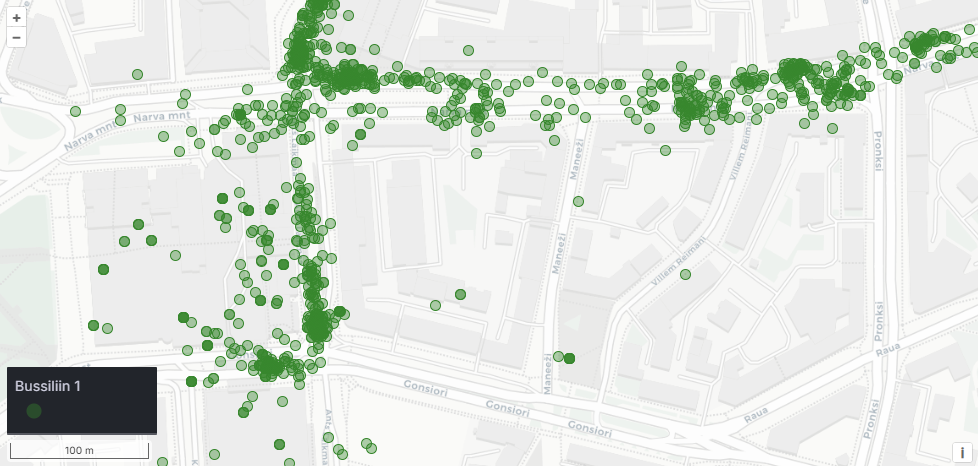
\includegraphics[width=.8\textwidth]{figures/gpsvead.png} % Includes an image from the specified path, setting the width to 50% of the text width
    \caption{Veaga asukohad Kesklinnas.} % Provides a caption for the figure, italicizing the text
    \label{fig:gpsnoise} % Sets a label for the figure to be referenced later 
\end{figure}

Joonisel \ref{fig:gpsnoise} on näha, et sõidukite asukohad võivad kohati näidata end majade peal ehk  kohtades, kuhu bussidel ligipääs puudub. Samuti on näha ebatäpseid mõõtmisi seoses Viru Keskuse maaaluse bussipeatusega. See raskendab täpsete mõõtmiste tegemist. Kuid sellegipoolest on müra sees võimalik näha, et enamus mõõtmisi jääb tänavavõrgustikule. Teatud meetoditega on võimalik andmete kvaliteeti tõsta. Näiteks kaardiga sobitamine (\textit{map matching}), kus sõidutee piiridest välja jäävad koordinaadid saab seostada olemasoleva lähimal oleva teega ja tõsta õigesse kohta, selleks on olemas omaette teegid nagu barefoot \cite{barefoot}. Iga päev kogutakse kokku ka liinide marsruudid ja seal ei lõigata kurve sirgeks. Maailmas on näiteid, kus on märgatud, et kui GNSS asukohad on teatud veaga, siis staatilised andmed nagu marsruut ei ole seda. Seda teadmist kasutati Buenos Airese ühistransporti analüüsides, kus kirjutati enda algoritm, mis seostab koordinaadi mitte terve teedevõrgustikuga, vaid konkreetse liini marsruudiga \cite{buenosAires}. Töös toodi välja, et see on oluliselt efektiivsem kui barefoot lahendus.

\begin{figure}[H] % h-here, if possible; H-here, definitely; t-top of the page; b-bottom of the page; p-page of floats
    \centering
    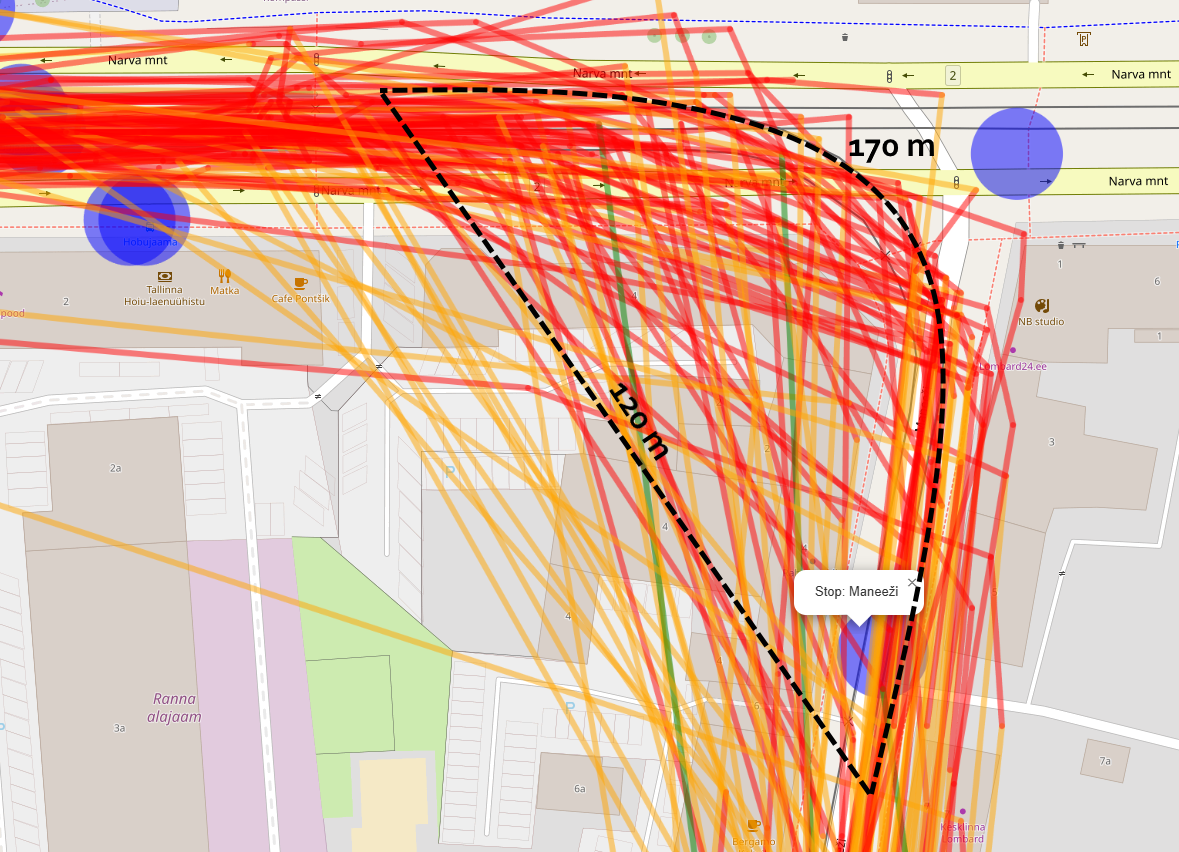
\includegraphics[width=.8\textwidth]{figures/Kurvsirgemaks.png} % Includes an image from the specified path, setting the width to 50% of the text width
    \caption{Trajektoorid lõikavad kurvi sirgemaks.} % Provides a caption for the figure, italicizing the text
    \label{fig:kurvsirgeks} % Sets a label for the figure to be referenced later
\end{figure}


Autor on siinse töö raames kogunud marsruutide andmeid ja kaalunud nende kasutamist täpsemate mõõtmiste saamiseks, kuid ei ole seda teinud suure töömahu tõttu.

Joonisel \ref{fig:kurvsirgeks} on näha, kuidas kiiruste arvutamisel ainult asukoha koordinaatidele tuginemine põhjustab olukordi, kus kurvid lõigatakse sirgemaks. Kuigi individuaalsed sektsioonid (sirge joon kahe mõõtmise vahel) näitavad õiget vahemaad, aega ja kiirust, siis sektsioonidest kokku pandud teekond võib hakata rohkete kurvide puhul vigast tulemust näitama. Reaalsuses on aga enamus marsruute suures osas võrdlemisi sirged  ja paljude kurvidega kohtades on ka ühistranspordi liikumiskiirused aeglasemad ja GNSS andmeid kogutakse läbitud vahemaa kohta rohkem kui sirgetel. See tähendab, et kurvide sirgeks lõikamine pole tegelikkuses nii suur probleem. Ning erinevalt eeltoodud Buenos Airesest, kus keskmiselt andis sõiduk oma asukohast teada iga 130 sekundi tagant ja ekstreemsematel juhtudel iga 10 minuti tagant, on Tallinna andmed palju järjepidevamad \cite{buenosAires}. Kiirused arvutatakse vaid siis, kui kahe andmepunkti vahe on 30 sekundit ehk 30 km/h liikuva sõiduki puhul keskmiselt iga 250 m tagant. Muid juhtumeid ignoreeritakse. See tähendab ka, et kaardile sobitamise algoritm ei ole hädavajalik. 
Peatükis \ref{section:valideerimine} analüüsiti erinevate liinide kiirusi ja leiti, et kurvide sirgeksvõtmise tõttu on keskmise kiiruse viga kuni 5\%. Autor pidas seda antud töö raames aksepteeritavaks, kuid edasiarenduste juures võiks sobitamise algoritmi rakendamist kaaluda.